\documentclass[a4paper,11pt]{article}
\pdfoutput=1 % if your are submitting a pdflatex (i.e. if you have
             % images in pdf, png or jpg format)

\usepackage{jheppub} % for details on the use of the package, please
                     % see the JHEP-author-manual
% Remove Prepared for submission to JHEP
\makeatletter
\def\@fpheader{\relax}
\makeatother

\usepackage[T1]{fontenc} % if needed

\usepackage{graphicx}
\usepackage{amsmath,amssymb,amsfonts}      
\usepackage{slashed}
\usepackage{hyperref}
\usepackage{graphicx,color}
\usepackage{colortbl}
\usepackage[usenames,dvipsnames,svgnames,table]{xcolor}
\definecolor{black}   {RGB}{0.0, 0.13, 0.28}
\definecolor{dukeblue}    {rgb}{0.0, 0.0, 0.61}
\usepackage{booktabs}
\newcommand{\ccell}{\cellcolor{dukeblue}}
\usepackage{multirow}
\usepackage[capitalize]{cleveref}
\usepackage{xfrac}
\usepackage{cancel}
\usepackage{xspace}
\usepackage[compat=1.1.0]{tikz-feynman}
\tikzfeynmanset{warn luatex=false}

\newcommand{\I}{\mathrm{i}}
\newcommand{\E}{\mathrm{e}}
\newcommand{\Lg}{\mathcal{L}}
\newcommand{\hn}{h}
\newcommand{\Hn}{{H^0}}
\newcommand{\An}{A^0}
\newcommand{\Hp}{{H^\pm}}
\newcommand{\smo}{\textsc{SModelS}\xspace}
\newcommand{\smodels}{\textsc{SModelS}\xspace}
\newcommand{\smothree}{\textsc{SModelS}~v3\xspace}
\newcommand{\smotwo}{\textsc{SModelS}~v2\xspace}
\newcommand{\smoone}{\textsc{SModelS}~v1\xspace}
\newcommand{\eg}{\textit{e.g.}}
\newcommand{\ie}{\textit{i.e.}}
\newcommand{\cf}{\textit{cf.}}
\newcommand{\calchep}{\textsc{CalcHep}}
\newcommand{\micromegas}{\textsc{micrOMEGAs}}
\newcommand{\Ztwo}{\ensuremath{{\mathcal Z}_2}}
\newcommand{\etmiss}{\ensuremath{{E_T^{\rm{miss}}}}}
\newcommand{\zp}{Z^{\prime}}
\newcommand{\zps}{Z^{\prime *}}
\newcommand{\zpm}{Z^{\prime \mu}}
\newcommand{\zpn}{Z^{\prime \nu}}

\newcommand{\main}[1]{{\color{red}#1}}
\newcommand{\be}{\begin{equation}}
\newcommand{\ee}{\end{equation}}
\newcommand{\bi}{\begin{itemize}}
\newcommand{\ei}{\end{itemize}}
\newcommand{\nn}{\nonumber}
\newcommand{\up}{\text{U(1)}^{\prime}}
\newcommand{\code}[1]{\texttt{#1}}
\newcommand{\GeV}{\mbox{ GeV}}


\newcommand{\comment}[1] {\textcolor{cyan}{\emph{#1}}}
\newcommand{\todo}[1] {\textcolor{red}{todo: \emph{#1}}}
\newcommand{\AL}[1] {\textcolor{blue}{#1}}
\newcommand{\SK}[1] {\textcolor{magenta}{#1}}
\newcommand{\TP}[1] {\textcolor{orange}{#1}}
\newcommand{\MMA}[1] {\textcolor{olive}{#1}}
\newcommand{\yox}[1] {\textcolor{teal}{#1}}
\newcommand{\CR}[1] {\textcolor{purple}{#1}}


% \input{diagrams}

%%%%%%%%%%%%%%%%%%%%%%%%%%%%%%%%%%%%%%%%%%%%%%%%%%%%
\title{\boldmath Dipole DM: Model Definitions}
%%%%%%%%%%%%%%%%%%%%%%%%%%%%%%%%%%%%%%%%%%%%%%%%%%%%

\author[a]{Andre~Lessa,} 
\author[b]{Jose~Zurita,}

\affiliation[a]{Centro de Ci\^encias Naturais e Humanas, Universidade Federal do ABC, Santo Andr\'e, 09210-580 SP, Brazil}

% e-mail addresses: one for each author, in the same order as the authors
\emailAdd{andre.lessa@ufabc.edu.br}


\begin{document} 
\maketitle
%\flushbottom

\tableofcontents


%%%%%%%%%%%%%%%%%%%%%%%%%%%%%%%%%%%%%%%%%%%%%%%%%%%%%%%%%%%%
\section{Dipole Dark Matter Model (\textsc{\small DipoleDM\_full\_UFO})}\label{sec:dipoleDM}
%%%%%%%%%%%%%%%%%%%%%%%%%%%%%%%%%%%%%%%%%%%%%%%%%%%%%%%%%%%%

The Dipole DM model extends the SM by adding two Dirac Fermions ($\chi_1$ and $\chi_0$) and a real scalar ($\phi$), all singlets under the SM gauge group.
The Lagrangian of the model is given by: 
\begin{equation}
    \mathcal{L} = \mathcal{L}_{\text{SM}} + \mathcal{L}_\phi + \mathcal{L}_\chi + \mathcal{L}_{\rm dipole} + \mathcal{L}_{H\chi}, 
    \label{eq:lagAll}
\end{equation}
where  $\mathcal{L}_{\text{SM}}$ represents the SM Lagrangian and
\begin{align}
   \mathcal{L}_{\phi} &=  \left(\partial^{\mu}\phi\right)^2 - \mu_2^2 |\phi|^2 - \lambda_2 \phi^4 - \lambda_3 \phi^2 |H|^2 \,, \label{eq:lagS}\\
   \mathcal{L}_\chi &=  i \overline{\chi}_i \cancel \partial \chi_i - \tilde{M}_{ij} \overline{\chi}_i \chi_j  - \left(y_\chi\right)_{ij} \overline{\chi}_i \chi_j \phi \,, \label{eq:lagChi}\\
   \mathcal{L}_{\rm dipole} &= \frac{\left(C_{\gamma \chi \chi}\right)_{ij}}{\Lambda} \overline{\chi}_i \sigma^{\mu\nu} \chi_j F_{\mu\nu} \,,\\
   \mathcal{L}_{H\chi} &= \frac{\left(C_{H \chi \chi}\right)_{ij}}{\Lambda} \overline{\chi}_i \chi_j |H|^2 \,.
\end{align}
In the equations above, $\sigma^{\mu\nu}= \frac{i}{2} \left[ \gamma^\mu,\gamma^\nu\right]$ and $H$ represents the Higgs doublet.


The model Lagrangian given in Eq.~\eqref{eq:lagAll} contains the scalar potential:
\begin{equation}
V_{H,\phi} = \mu_1^2 |H|^2 + \lambda_1 |H|^4  + \mu_{2}^2 \phi^2 + \lambda_2 \phi^4 + \lambda_3 \phi^2 |H|^2 \,.
\end{equation}
Assuming that both $H$ and $\phi$ develop vevs, $\langle \phi \rangle = v_D/\sqrt{2}$ and $\langle H \rangle = v/\sqrt{2}$, we obtain the mass eigenstates $h$ and $S$:
\begin{align}
	h &= (\sqrt{2} H^0 -v) \cos \alpha - (\sqrt{2} \phi-v_D) \sin \alpha \,,  \nonumber\\
	S &= (\sqrt{2} \phi - v_D) \cos \alpha + (\sqrt{2} H^0 - v) \sin \alpha \,. \label{eq:alpha}
\end{align}
Where the mixing angle ($\alpha$) is given by
\begin{equation}
	\tan(2 \alpha) \equiv \frac{\lambda_{3} v v_D}{\lambda_1 v^2-\lambda_2 v_D^2}\,.
	\label{tan}
\end{equation}
and with masses: 
\begin{equation}
m_{S,h}^2 = \lambda_{1} v^2+\lambda_{2} v_D^2 \mp \left(\lambda_{1} v^2-\lambda_{2} v_D^2\right) \sqrt{1 + \tan^2(2 \alpha)}\,,
   \label{mhs}
\end{equation}
Using the above equations, we can express the quartic couplings ($\lambda_i$) and the mass parameters ($\mu_i$) in terms of the physical masses, mixing angle and vevs:  
\begin{align}
 \lambda_1 &=  \frac{1}{2 v^2}\left(\cos^2\alpha\, m_{h}^2+m_{S}^2 \sin^2\alpha\right),\\
 \lambda_2 &= \frac{1}{2 v_D^2} \left(\cos^2\alpha \, m_{S}^2+ m_{h}^2 \sin^2 \alpha\right),\\
  \lambda_{3} &= \frac{1}{v_D v} \left(m_{S}^2 -m_h^2 \right) \sin\alpha \cos\alpha \; ,\\
  \mu_1^2 &=  -\left(\lambda_{1}v^2 + \lambda_{3} \frac{v_D^2}{2} \right), 
  \quad\\
  \mu_2^2 &= -\left(\lambda_{2} v_D^2 + \lambda_{3}\frac{v^2}{2}\right)
\end{align}
Therefore, the parameters of the scalar potential ($\mu_{1,2}$ and $\lambda_{1,2,3}$) can be replaced by $m_{h},m_S,v,v_D$ and $\sin\alpha$.

Finally, the dark fermion mass matrix $\tilde{M}_{ij}$ is defined in the mass eigenstate basis:
\begin{equation*}
	\tilde{M}_{ij} = M_i \delta_{ij} -\frac{v_D}{\sqrt{2}} (y_{\chi})_{ij} - \frac{v^2}{2\Lambda} (C_{H\chi\chi})_{ij}
\end{equation*}
where $M_i$ are the physical masses.

In addition to the Lagragian in \cref{eq:lagAll}, the effective $h-G-G$ and $S-G-G$ couplings induced by a top quark loop were also included as effective operators:

\begin{equation*}
	\mathcal{L}_{GG\phi} =  \frac{g_s^2}{48 \pi^2 v} \cos\alpha F(m_h^2/m_t^2) G^{\mu\nu} G_{\mu\nu} h + \frac{g_s^2}{48 \pi^2 v} \sin\alpha F(m_S^2/m_t^2) G^{\mu\nu} G_{\mu\nu} S
\end{equation*}
where $F(x)$ is the effective loop function.
\subsection*{Model Parameters}

The model parameters are given in \cref{tab:parameters} as well as their naming convention in the UFO model and their default values. The $C_{\gamma \chi\chi}$ and $C_{H \chi\chi}$ matrices are assumed to be real and symmetric.


\begin{table}[h!]   \centering
	\rowcolors{2}{gray!10}{white}
	\vspace{0.2cm}
	\caption{Model parameters, their respective names in the UFO model and default values.\label{tab:parameters}}
	\begin{tabular}{p{2cm}|p{3cm}|p{3cm}}
		\toprule
		\textbf{Parameter} & \textbf{UFO name} & \textbf{Default Value}\\ \toprule 
		$\Lambda$  & LambdaUV & 5 TeV\\
		$(C_{\gamma \chi\chi})_{11}$  & Caxx1 & 0\\
		$(C_{\gamma \chi\chi})_{00}$  & Caxx0 & 0\\
		$(C_{\gamma \chi\chi})_{10}$  & Caxx10 & 0.1\\
		$(C_{H \chi\chi})_{11}$  & Chxx1 & 0\\
		$(C_{H \chi\chi})_{00}$  & Chxx0 & 0\\
		$(C_{H \chi\chi})_{10}$  & Chxx10 & 0.1\\
		$(y_\chi)_{11}$  & ychi1 & 1.0\\
		$(y_\chi)_{00}$  & ychi0 & 0\\
		$(y_\chi)_{10}$  & ychi10 & 0\\
		$\sin\alpha$  & sina & 0.2\\
		$v_D$  & vevD & 1 TeV\\
		$m_S$ & MSd & 1.5 TeV\\ 
		$M_0$ & M0 & 425 GeV\\
		$M_1$ & M1 & 500 GeV\\
		\bottomrule        
	\end{tabular}
\end{table}


\subsection*{Feynman rules}

The relevant Feynman rules for the BSM particles are given in \cref{tab:feynmanRules} below. Here, $f$ represents any of the SM fermions and $q$ any SM quark.

\begin{table}[h!]   \centering
    \rowcolors{2}{gray!10}{white}
    \vspace{0.2cm}
    \begin{tabular}{p{2cm}|p{8.5cm}}
      \toprule
      \textbf{Interaction} & \textbf{Vertex term}\\ \toprule 
      $\chi_i\,\chi_j\,h$  & $ \frac{i}{\sqrt{2}} (y_{\chi})_{ij} \sin\alpha -i \frac{v}{\Lambda} (C_{H\chi\chi})_{ij} \cos\alpha $\\
      $\chi_i\,\chi_j\, A^\mu$  & $-i \frac{1}{\Lambda} (C_{\gamma\chi\chi})_{ij} (\gamma^\mu \slashed{p} - \slashed{p} \gamma^\mu)$\\
      $S\,\chi_i\,\chi_j$  & $ -\frac{i}{\sqrt{2}} (y_{\chi})_{ij} \cos\alpha -i \frac{v}{\Lambda} (C_{H\chi\chi})_{ij} \sin\alpha $\\      
      $S\,h\,h$  & $- i \frac{m_{S}^{2}}{2 v}  \left( 1 + 2 \frac{m_{h}^{2}}{m_{S}^{2}}\right)  \left( \cos\alpha + 2 \frac{v}{v_D} \sin\alpha \right)  \sin (2\alpha)$\\
      $S\,f\,\bar{f}$  & $-i \frac{m_f}{v} \sin\alpha$ \\      
      $S\,W_\mu^-\,W_\nu^+$  & $2 i g^{\mu\nu} \frac{m_{W}^2}{v} \sin\alpha$\\
      $S\,Z_\mu\,Z_\nu$  & $2 i g^{\mu\nu} \frac{m_{Z}^2}{v} \sin\alpha$\\
      $S\,G_\mu\,G_\nu$  & $i \frac{g_s^2}{12 \pi^2 v} \sin\alpha F(m^2_S/m^2_t) (p_1^\mu p_2^\nu - g^{\mu\nu} p_1\cdot p_2) $\\
      \bottomrule        
    \end{tabular}
    \caption{Feynman rules for the relevant interactions in the full model. \label{tab:feynmanRules}}
\end{table}

The production of $S$ at the LHC mainly occurs due to gluon-fusion and is proportional to $\sin\alpha$. 
In \cref{fig:xsec_s} we show the $\sigma(p p \to S)$ as a function of $m_S$ for $\sin\alpha = 0.2$ and a center of mass energy of 13.6 TeV.

\begin{figure}
	\centering
	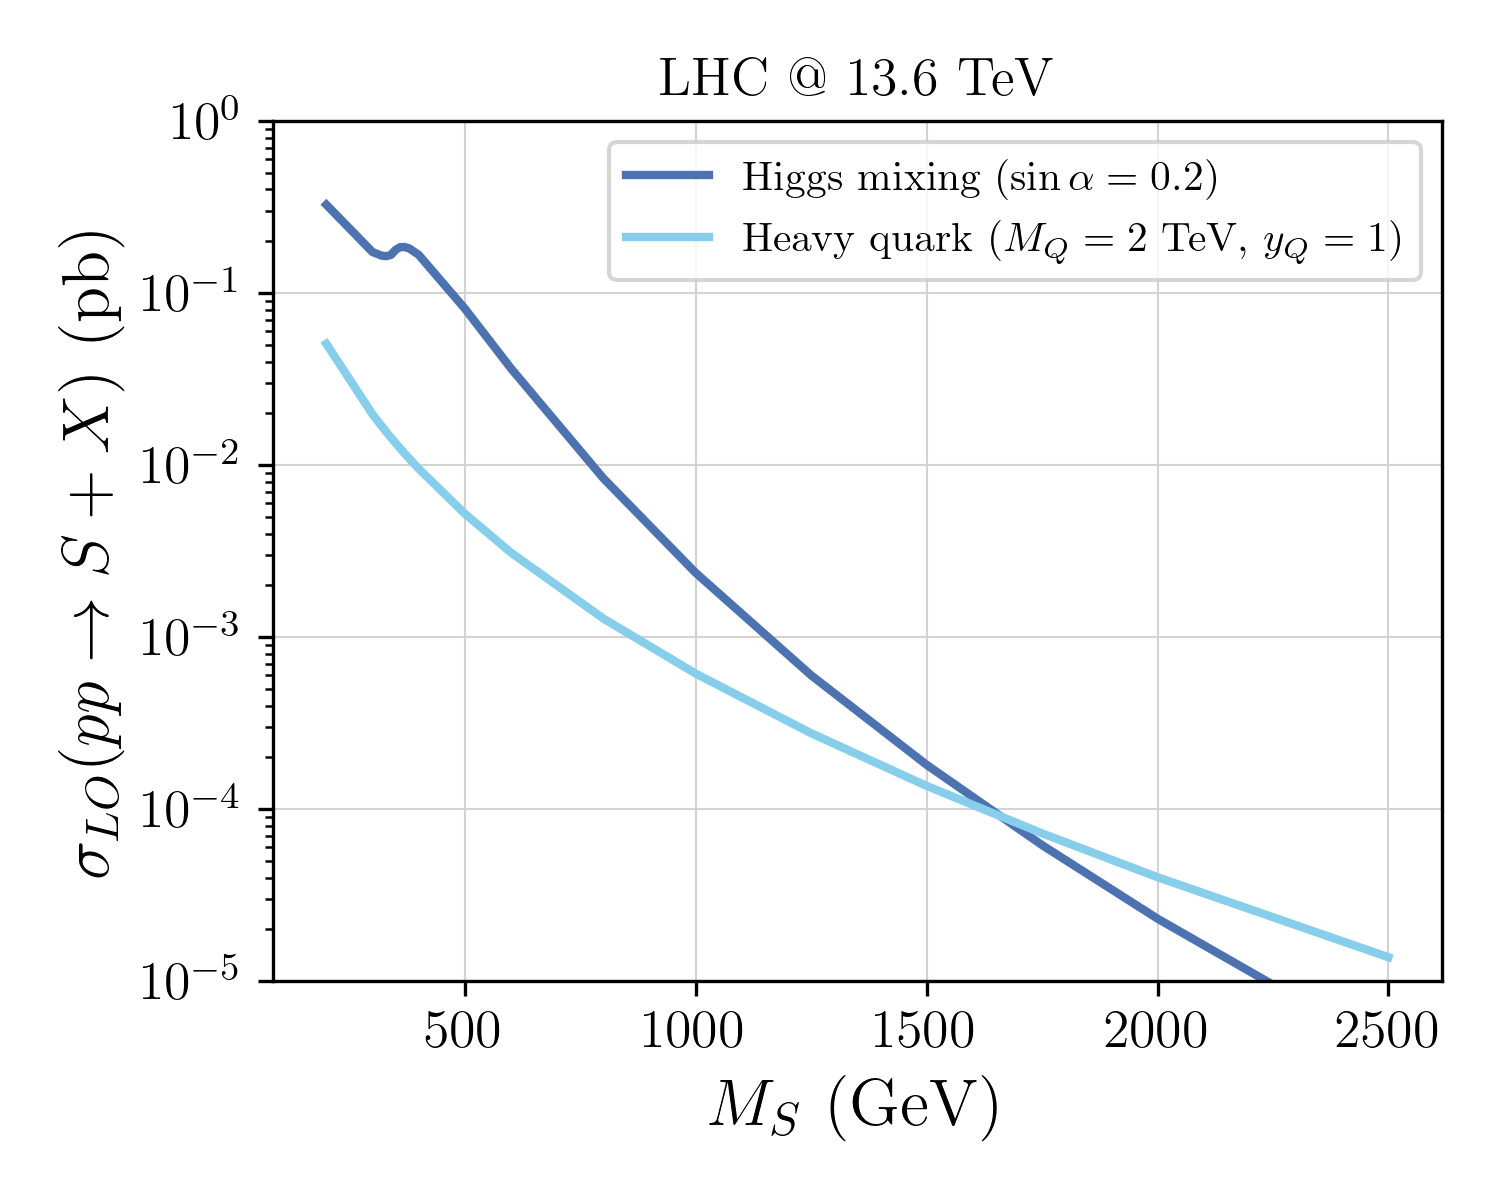
\includegraphics[scale=0.7]{../../xsecs_mS.png}
	\caption{Production cross-section for the dark scalar $S$ as a function of its mass.} \label{fig:xsec_s}
\end{figure}

\newpage
\clearpage
\subsection{Minimal Couplings to Higgs (\textsc{\small DipoleDM\_minimalH\_UFO})}

The minimal scenario assumes that $\chi_0$ only couples through the $H$ effective operator and the diagonal entries are zero:
\begin{align}
	(C_{\gamma\chi\chi})_{ij} &= 0\\
	(C_{H\chi\chi})_{ij} &= 0 \mbox{ , if $i = j$} \\
	(y_{\chi})_{ij} & = 0 \mbox{ , if $i = 0$ or $j = 0$ }
\end{align}
With the above assumptions the Lagrangian simplifies to:
\begin{equation}
	\mathcal{L}_{\chi} =  i \overline{\chi}_i \cancel \partial \chi_i - \tilde{M}_{ij} \overline{\chi}_i \chi_j - \left(y_\chi\right)_{11} \overline{\chi}_1 \chi_1 \phi + \frac{\left(C_{H \chi \chi}\right)_{01}}{\Lambda} \left( \overline{\chi}_0 \chi_1 |H|^2 + h.c.\right)
\end{equation}
resulting in the vertices given in \cref{tab:feynmanRulesH}.

\begin{table}[h!]   \centering
	\rowcolors{2}{gray!10}{white}
	\vspace{0.2cm}
	\begin{tabular}{p{2cm}|p{8.5cm}}
		\toprule
		\textbf{Interaction} & \textbf{Vertex term (Minimal H)}\\ \toprule 
		$h\, \chi_1\,\chi_1$ & $\frac{i}{\sqrt{2}} (y_{\chi})_{11} \sin\alpha$\\
		$S\,\chi_1\,\chi_1$  & $-\frac{i}{\sqrt{2}} (y_{\chi})_{11} \cos\alpha $\\
		$\chi_1\,\chi_0\,h$  & $-i \frac{v}{\Lambda} (C_{H\chi\chi})_{01} \cos\alpha$\\
		$S\,\chi_1\,\chi_0$ &  $-i \frac{v}{\Lambda} (C_{H\chi\chi})_{01} \sin\alpha$\\
    	$S\,G_\mu\,G_\nu$  & $i \frac{g_s^2}{12 \pi^2 v} \sin\alpha F(m^2_S/m^2_t) (p_1^\mu p_2^\nu - g^{\mu\nu} p_1\cdot p_2) $\\
		\bottomrule        
	\end{tabular}
	\caption{Feynman rules for the relevant interactions in the {\bf minimal} model with couplings to Higgs. The couplings between $S$ and two SM particles are the same as in \cref{tab:feynmanRules} and have been omitted. \label{tab:feynmanRulesH}}
\end{table}


In this scenario the heavy fermion can only decay through the effective operator, hence:
\begin{align}
	\Gamma (\chi_1 \to h \chi_0) & = \cos^2\alpha \frac{C_{H\chi\chi}^2}{16 \pi} \frac{v^2}{\Lambda^2} M_1 \left[\left(1 + \frac{M_0}{M_1}\right)^2 - \frac{m_h^2}{M_1^2} \right]  \sqrt{\lambda\left(1,\frac{M_0^2}{M_1^2},\frac{m_h^2}{M_1^2}\right)}\\
	\Gamma (\chi_1 \to S \chi_0) & = \sin^2\alpha \frac{C_{H\chi\chi}^2}{16 \pi} \frac{v^2}{\Lambda^2} M_1 \left[\left(1 + \frac{M_0}{M_1}\right)^2 - \frac{m_S^2}{M_1^2} \right]  \sqrt{\lambda\left(1,\frac{M_0^2}{M_1^2},\frac{m_S^2}{M_1^2}\right)}\, ,
\end{align} 
where $\lambda(x,y,z) = x^2 + y^2 + z^2 + 2 x y + 2 x z + 2 y z$.


Note that the decay to $S + \chi_0$ is suppressed by $\sin\alpha$ and will be subdominant as long as $m_h \lesssim m_S$.
Furthermore, if $\Delta m = m_{\chi_1} - m_{\chi_0}  < m_h$ the decay is kinematically suppressed and takes place through an off-shell Higgs ($h^*$). In \cref{fig:chi1_decayH} we show the branching ratios as a function of $\Delta m$ for $m_{\chi_1} = 500$ GeV.
For the extremely compressed scenario ($\Delta m < 2$ GeV) only the decay to gluons ($h^* \to g g$) is kinematically allowed, resulting in a 100\% BR in this channel. Once decays to $\tau$s are allowed, they become the dominant channel. For $\Delta m \gtrsim 10$~GeV the decays $h^* \to b \bar{b}$ are open and rapidly become the main decay channel up to $\Delta m > m_h$, where the decay is 100\% to an on-shell Higgs.
Finally, in \cref{fig:chi1_lifetimeH} we show the decay length as a function of $\Delta m$, where we see that it can take a wide range of values depending on the mass compression. In particular, once the $b \bar{b}$ channel is open the decay length falls below 10~m. It is important to notice, however, that the lifetime scales as  $\tau \propto \left(\Lambda/C_{H\chi\chi}\right)^2$ and will be further suppressed for larger values of $\Lambda/C_{H\chi\chi}$.

\begin{figure}
	\centering
	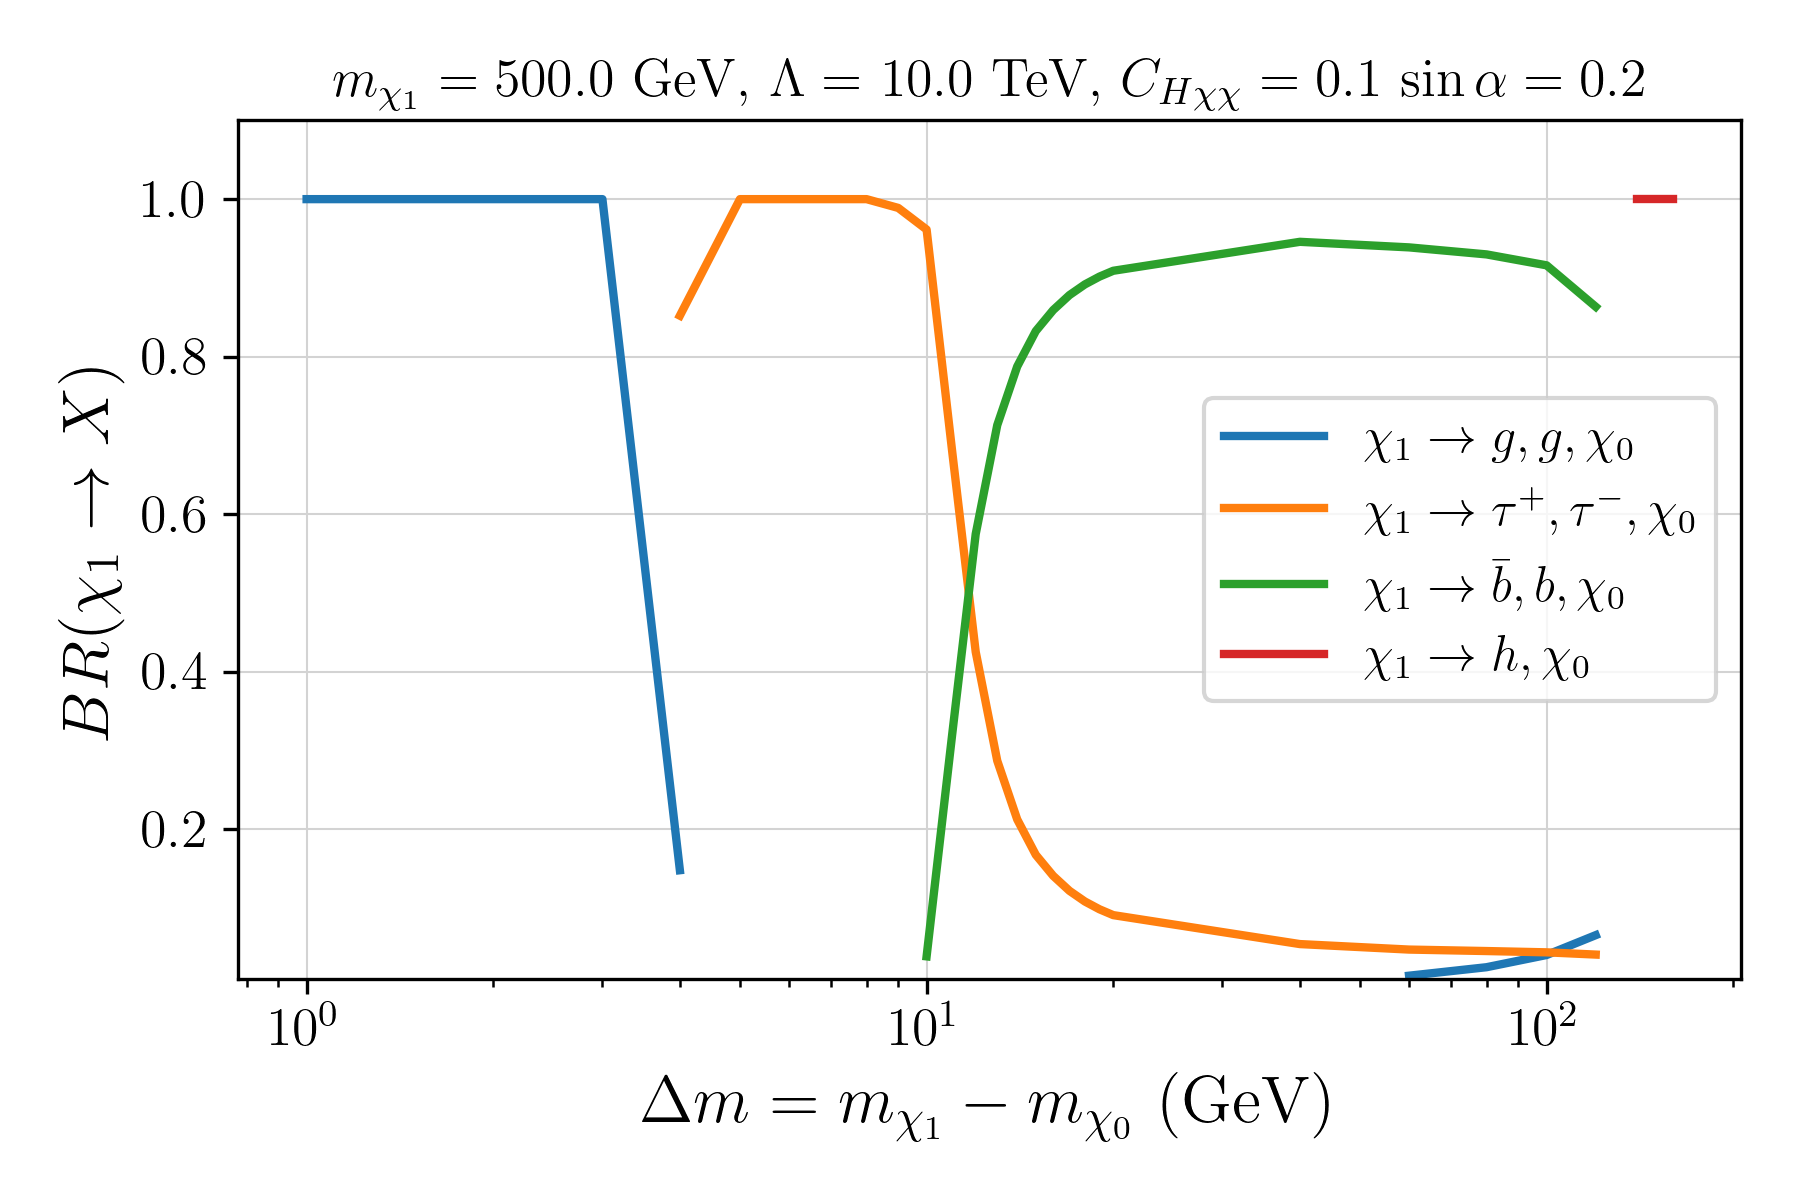
\includegraphics[scale=0.8]{../../chi1_BRs_H.png}
	\caption{Branching ratios for $\chi_1$ decays in the minimal H scenario as a function of $\Delta m = m_{\chi_1} - m_{\chi_0}$. Only channels with a branching ratio larger than 1\% are shown.} \label{fig:chi1_decayH}
\end{figure}

\begin{figure}
	\centering
	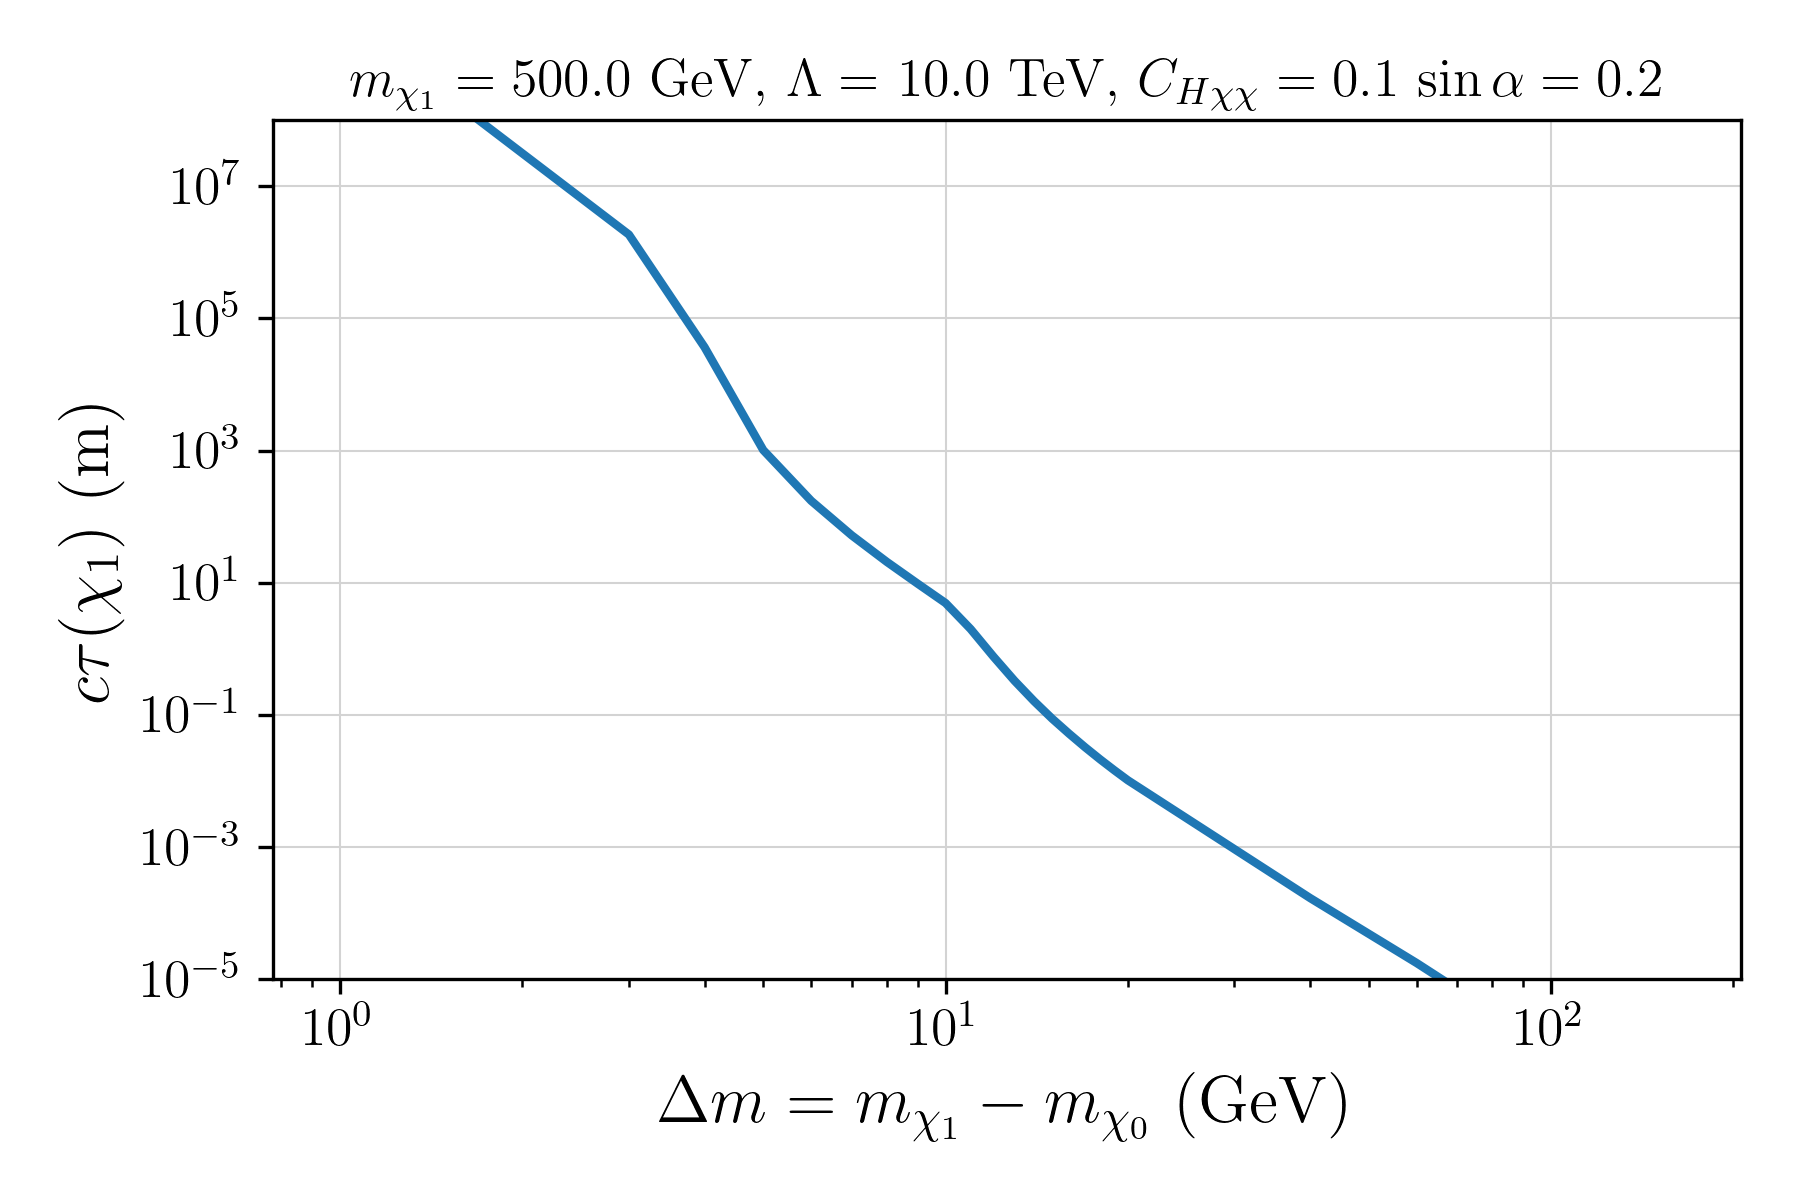
\includegraphics[scale=0.8]{../../chi1_lifetime_H.png}
	\caption{Proper decay length for $\chi_1$ in the minimal H scenario as a function of $\Delta m = m_{\chi_1} - m_{\chi_0}$.} \label{fig:chi1_lifetimeH}
\end{figure}

\subsection{Minimal Couplings to Photon (\textsc{\small DipoleDM\_minimalA\_UFO})}

The minimal scenario assumes that $\chi_0$ only couples through the $F^{\mu\nu}$ effective operator and the diagonal entries are zero:
\begin{align}
	(C_{\gamma\chi\chi})_{ij} &= 0 \mbox{ , if $i = j$} \\
	(C_{H\chi\chi})_{ij} &= 0\\
	(y_{\chi})_{ij} & = 0 \mbox{ , if $i = 0$ or $j = 0$ }
\end{align}
With the above assumptions the Lagrangian simplifies to:
\begin{equation}
	\mathcal{L}_{\chi} =  i \overline{\chi}_i \cancel \partial \chi_i - \tilde{M}_{ij} \overline{\chi}_i \chi_j - \left(y_\chi\right)_{11} \overline{\chi}_1 \chi_1 \phi + \frac{\left(C_{\gamma \chi \chi}\right)_{01}}{\Lambda} \left(\overline{\chi}_0 \sigma^{\mu\nu} \chi_1 + h.c.\right) F_{\mu\nu} 
\end{equation}
resulting in the vertices given in \cref{tab:feynmanRulesA}.

\begin{table}[h!]   \centering
	\rowcolors{2}{gray!10}{white}
	\vspace{0.2cm}
	\begin{tabular}{p{2cm}|p{8.5cm}}
		\toprule
		\textbf{Interaction} & \textbf{Vertex term (Minimal A)}\\ \toprule 
		$ h\,\chi_1\,\chi_1$ & $\frac{i}{\sqrt{2}} (y_{\chi})_{11} \sin\alpha$\\
		$S\,\chi_1\,\chi_1$  & $-\frac{i}{\sqrt{2}} (y_{\chi})_{11} \cos\alpha $\\
		$\chi_1\,\chi_0\, A^\mu$  & $-i \frac{1}{\Lambda} (C_{\gamma\chi\chi})_{01} (\gamma^\mu \slashed{p} - \slashed{p} \gamma^\mu)$\\
		$S\,G_\mu\,G_\nu$  & $i \frac{g_s^2}{12 \pi^2 v} \sin\alpha F(m^2_S/m^2_t) (p_1^\mu p_2^\nu - g^{\mu\nu} p_1\cdot p_2) $\\
		\bottomrule        
	\end{tabular}
	\caption{Feynman rules for the relevant interactions in the {\bf minimal} model with couplings to photons. The couplings between $S$ and two SM particles are the same as in \cref{tab:feynmanRules} and have been omitted. \label{tab:feynmanRulesA}}
\end{table}


In this scenario the heavy fermion can only decay through the effective operator, hence:
\begin{equation}
	\Gamma (\chi_1 \to \gamma \chi_0) = \frac{C_{\gamma\chi\chi}^2}{2 \pi} \frac{M_1^2}{\Lambda^2} M_1 \left(1-\frac{M_0^2}{M_1^2}\right)^3
\end{equation} 

Since this is the only allowed channel it has always 100\% branching ratio and the lifetime for the compressed scenario is given by:
\begin{equation}
	c \tau = 1.55 \times 10^{-6} \mbox{ m} \left(\frac{0.1}{C_{\gamma\chi\chi}}\right)^2 \left(\frac{\Lambda}{10\mbox{ TeV}}\right)^2 \left(\frac{1 \mbox{ GeV}}{\Delta m}\right)^{3}\, ,
\end{equation}
where we have assumed $M_0 \lesssim M_1$, so $\Delta m^2 = M_1^2 - M_0^2 \simeq 2 M_1 \Delta m$. In \cref{fig:chi1_lifetimeA} we show the decay length as a function of $\Delta m$. As we can see, even for $\Lambda = 100$~TeV the decay is prompt as long as $\Delta m > 1$~GeV.

\begin{figure}
	\centering
	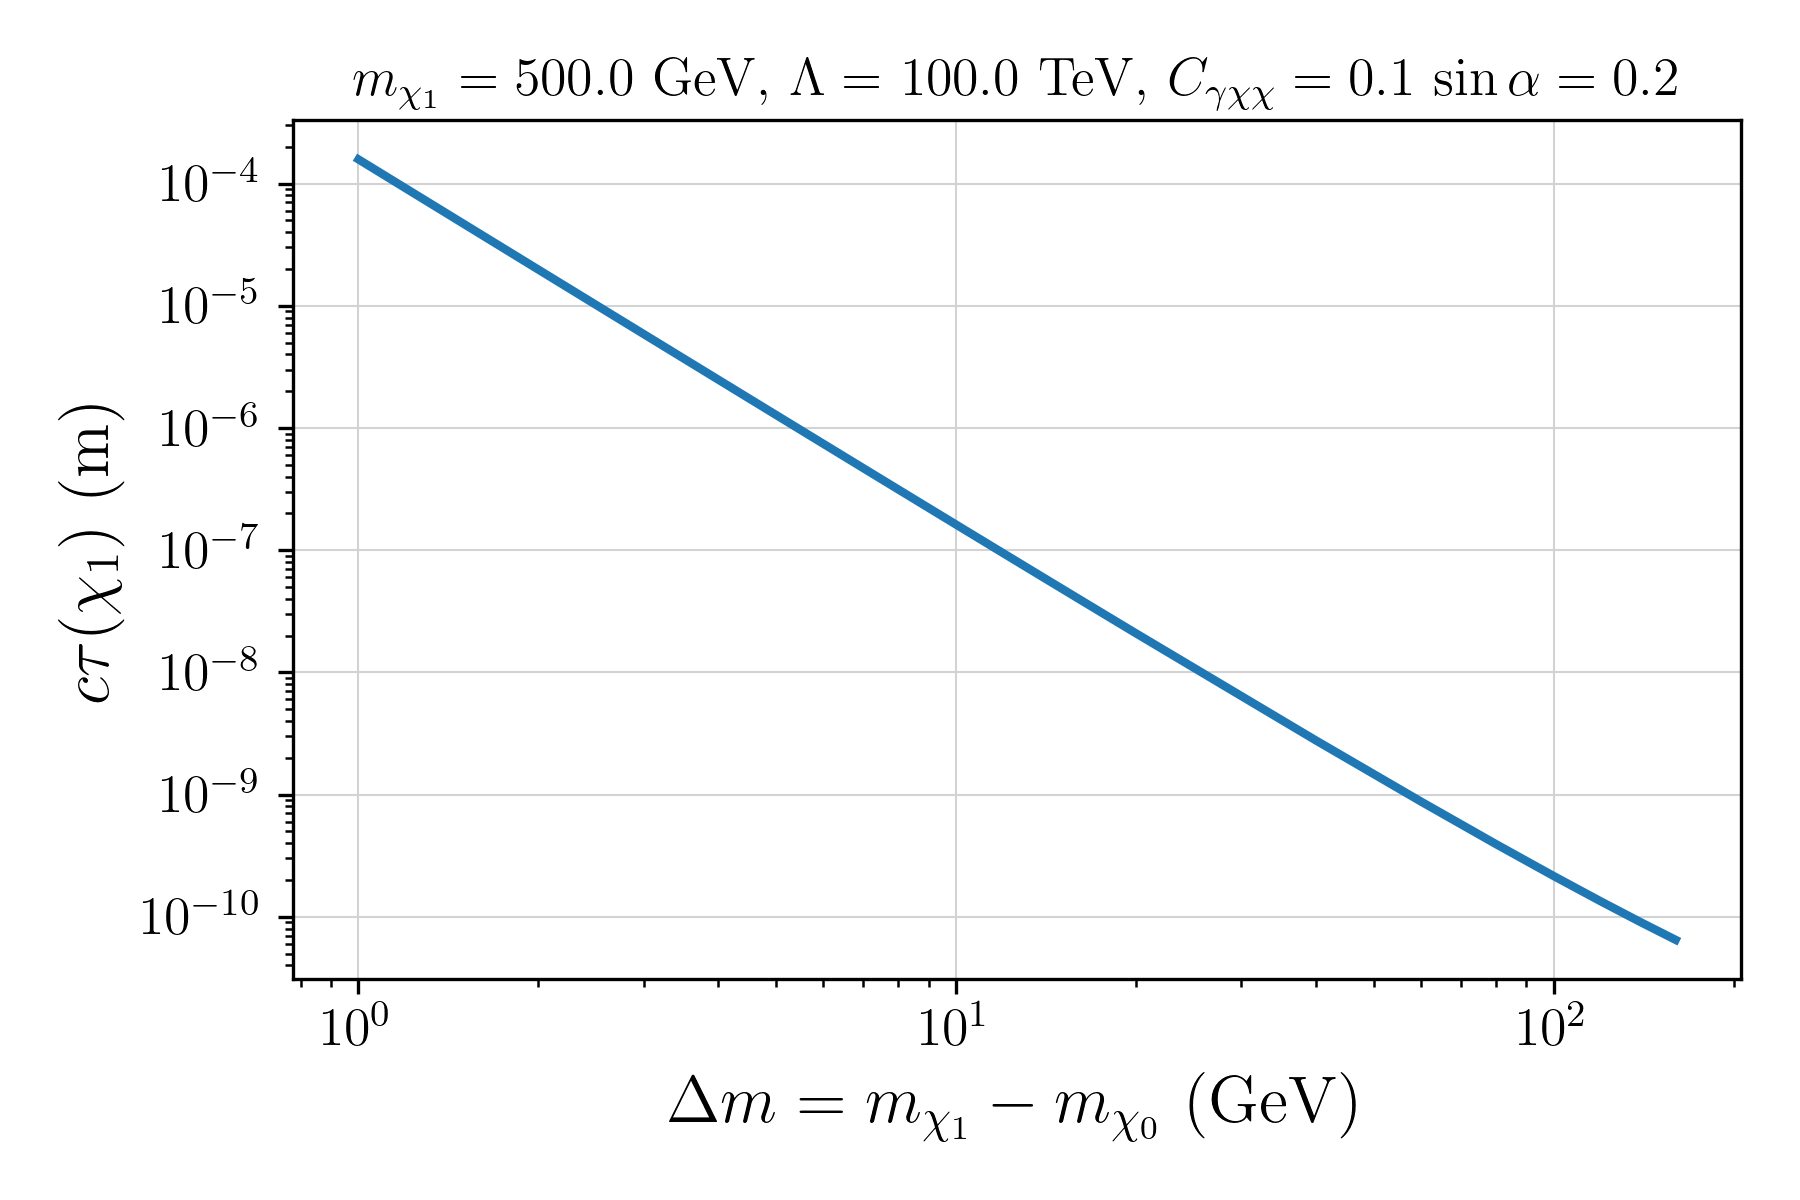
\includegraphics[scale=0.8]{../../chi1_lifetime_A.png}
	\caption{Proper decay length for $\chi_1$ in the minimal photon scenario as a function of $\Delta m = m_{\chi_1} - m_{\chi_0}$.} \label{fig:chi1_lifetimeA}
\end{figure}

%\clearpage
%\bibliographystyle{JHEP}
%\bibliography{references}


\end{document}
